%Author: Michael Bucher
\section{Access Terminal}\label{design:access-terminal}
The access terminal is the frontend component in the proposed access control solution in subsection \ref{subsection:access-control}. It is intended to be used on a tablet to display a QR code that contains the necessary information for the guest to validate the held tickets to enter the location.

The application is structured into two views. The connection view as shown in figure \ref{img:terminal-registration-form} contains a form to register the terminal with the set up backend. The required information is the base URL of the host backend, the secret that is stored in the backend to permit this device and the area where the guest is coming from and the area where the guest will be after passing the terminal. Currently there are five different areas provided, whereas the area \textit{entrance} must be used initially when a guest enters the location the first time. Finally, when the registration was successful, the application routes to the terminal view.

\begin{figure}[H]
    \centering
    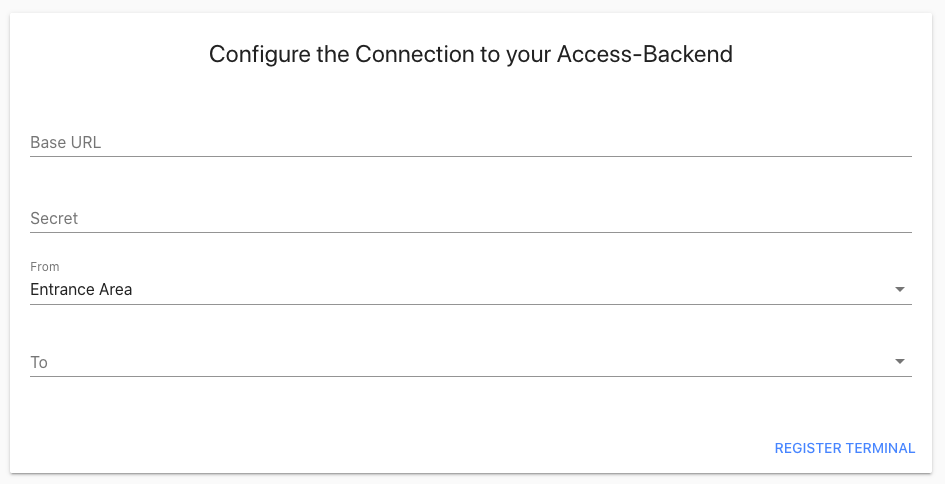
\includegraphics[width=15cm]{images/terminal-registration.png}
    \caption{Terminal Registration Form \protect}
    \label{img:terminal-registration-form}
\end{figure}

The terminal shows a QR code that contains a random message and the base URL of the backend. Whenever a guest requests the verification of its signature connected to this terminal the status changes to either \textit{granted} or \textit{denied}. Depending on that status a green or a red field is displayed on the terminal. Upon a click the terminal requests a new random message which also resets the status in the backend. This message is then displayed in a new QR code and the terminal awaits again a status change.
